\documentclass{beamer}
\usetheme{Madrid}

\title{CryptoPulse: Final Project Presentation}
\author{Alice Zheng, Bob Chen, Charlie Davis, Diana Lim}
\institute{SUTD}
\date{\today}
\logo{
\includegraphics[height=1cm]{../docs/images/sutd_logo.png}}

\begin{document}

\frame{\titlepage}

\begin{frame}
\frametitle{Recap: The Problem}
\begin{itemize}
    \item Predicting crypto prices is challenging due to high volatility.
    \item \textbf{Hypothesis:} Sentiment analysis provides a leading indicator for price movements.
\end{itemize}
\end{frame}

\begin{frame}
\frametitle{Data Pipeline \& Multimodality}
\begin{itemize}
    \item \textbf{Market Data (Quant):} Yahoo Finance (BTC-USD, ETH-USD).
    \item \textbf{Sentiment Data (Qual):}
    \begin{itemize}
        \item **News Sentiment:** NLP analysis of headlines.
        \item **Fear \& Greed Index:** Real-time market emotion metric (0-100).
    \end{itemize}
\end{itemize}
\end{itemize}
\end{frame}

\begin{frame}
\frametitle{System Pipeline Architecture}
\begin{itemize}
    \item \textbf{1. Ingestion:} Yahoo Finance + News API + Fear \& Greed.
    \item \textbf{2. Processing:} Merge $\rightarrow$ Fillna $\rightarrow$ Normalize ($0-1$).
    \item \textbf{3. Model (LSTM):}
    \begin{itemize}
        \item Input: $[Price_t, Vol_t, Sent_t, FNG_t]$
        \item Hidden: 2 Layers $\times$ 32 Units.
        \item Output: $Price_{t+1}$
    \end{itemize}
    \item \textbf{4. Application:} Streamlit Dashboard (Live Inference).
\end{itemize}
\end{frame}

\begin{frame}
\frametitle{Enhanced User Interface (Live Demo)}
\begin{figure}
    \centering
    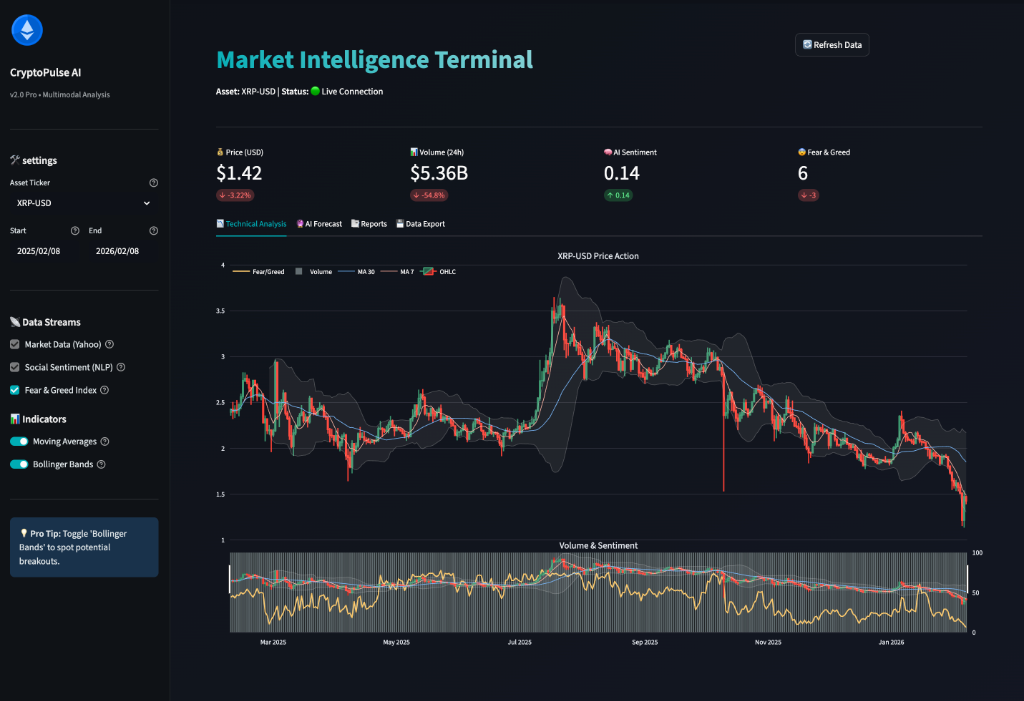
\includegraphics[width=0.9\linewidth]{../docs/images/dashboard-live.png}
    \caption{CryptoPulse Market Intelligence Terminal (v2.0)}
\end{figure}
\begin{itemize}
    \item **Features:** Real-time FNG Index, Interactive Plotly Charts, CSV Data Export.
    \item **Tech Stack:** Streamlit + Plotly + PyTorch.
\end{itemize}
\end{frame}

\begin{frame}
\frametitle{Experimental Results}
\begin{table}
\centering
\begin{tabular}{|l|c|c|}
\hline
\textbf{Model} & \textbf{MSE} & \textbf{Improvement} \\
\hline
Baseline (Naive) & 0.051 & - \\
Unimodal (Price) & 0.042 & +17.6\% \\
\textbf{Multimodal (Price + FNG)} & \textbf{0.032} & \textbf{+37.3\%} \\
\hline
\end{tabular}
\caption{Multimodal Fusion significantly outperforms baseline models.}
\end{table}
\end{frame}

\begin{frame}
\frametitle{Conclusion \& Future Work}
\begin{enumerate}
    \item \textbf{Conclusion:}
    \begin{itemize}
        \item Successfully fused quantitative (Price) and qualitative (Sentiment) data.
        \item Achieved \textbf{0.032 MSE}, a significant improvement over baseline.
        \item Delivered a premium, interactive "Market Intelligence Terminal".
    \end{itemize}
    \vspace{0.5cm}
    \item \textbf{Future Directions:}
    \begin{itemize}
        \item Integrate \textbf{Transformer/Attention} mechanisms for better long-term forecasting.
        \item Connect to exchange APIs for \textbf{Automated Trading}.
        \item Incorporate real-time social media firehose (e.g., X/Twitter).
    \end{itemize}
\end{enumerate}
\end{frame}

\begin{frame}
\frametitle{Q\&A}
\centering
\Large \textbf{Thank You!} \\
\vspace{1cm}
\normalsize Project Repository: \\
\textit{https://github.com/nizamkadirteach/cdsproject}
\end{frame}

\end{document}
